\documentclass[aspectratio=169,11pt]{beamer}

\usepackage{fontspec}
\usepackage{polyglossia}
\setdefaultlanguage{portuguese}
\usepackage{graphicx}
\usepackage{booktabs}
\usepackage{listings}
\usepackage{xcolor}
\usepackage{animate}

\graphicspath{{figures/}}

\usetheme{default}
\setbeamertemplate{navigation symbols}{}
\setbeamertemplate{footline}[frame number]
\setbeamercolor{frametitle}{fg=black}
\setbeamerfont{frametitle}{series=\bfseries}
\setbeamercolor{structure}{fg=black!70}

\definecolor{codebg}{gray}{0.95}
\lstset{
  language=C++,
  basicstyle=\ttfamily\scriptsize,
  keywordstyle=\color{blue!60!black}\bfseries,
  commentstyle=\color{gray},
  backgroundcolor=\color{codebg},
  frame=none,
  columns=fullflexible,
  keepspaces=true,
  morekeywords={__global__,__device__,__host__,__shared__,__syncthreads,atomicAdd,curand_init},
}

\newcommand{\aaa}[1]{\textcolor{orange!90!black}{\textbf{[A30: #1]}}}

\title{CUDA: programando a GPU}
\subtitle{e dois projetos: a agulha de Buffon (EP3) e a estrela manchada (EP4)}
\author{Welton}
\institute{AGA 511 · Métodos Computacionais em Astronomia · IAG/USP}
\date{24 de novembro de 2026}

\begin{document}

\begin{frame}
  \titlepage
\end{frame}

% ============================================================ 0. história e usos → os conceitos

\begin{frame}{Por que existe uma GPU?}
  \centering\Large
  Cada parte de uma GPU responde a um problema que alguém teve.\\[1em]
  \normalsize A história explica a arquitetura.
\end{frame}

\begin{frame}{Ciência e indústria, juntas}
  \begin{itemize}
    \item o paralelismo nasceu na \textbf{ciência}: computadores vetoriais (Cray-1, 1976), milhares de processadores simples fazendo a mesma coisa (Connection Machine, 1985)
    \item foi para a \textbf{indústria}: placas de vídeo para jogos, nos anos 1990
    \item voltou para a ciência, e hoje as duas andam \textbf{juntas}: supercomputadores, IA, simulação
  \end{itemize}
  \vfill
  \textbf{CUDA} é a plataforma desses últimos 20 anos, e provavelmente de boa parte dos próximos.
\end{frame}

\begin{frame}{1999: desenhar milhões de pixels por quadro}
  \begin{itemize}
    \item GeForce 256 (1999): um \emph{pipeline} fixo de gráficos
    \item cada pixel é calculado de forma \textbf{independente} dos outros
    \item muitas unidades simples em vez de poucas unidades rápidas
  \end{itemize}
  \vfill
  \textbf{O conceito:} paralelismo de dados; \textbf{vazão} (\emph{throughput}) em vez de \textbf{latência}
\end{frame}

\begin{frame}{2001--2006: um programa por pixel, e os cientistas pegam carona}
  \begin{itemize}
    \item \emph{shaders} programáveis (GeForce 3, 2001): um pequeno programa roda uma vez por pixel
    \item GPGPU (BrookGPU, 2004): matrizes disfarçadas de texturas para fazer ciência
  \end{itemize}
  \vfill
  \textbf{Os conceitos:} o \textbf{kernel}; e por que faltava um modelo de programação de verdade
\end{frame}

\begin{frame}{2006--2007: CUDA}
  \begin{itemize}
    \item \emph{shaders} unificados (G80, 2006): núcleos iguais, agrupados em \textbf{multiprocessadores} (SMs)
    \item CUDA: programar a GPU em C, sem fingir que é gráfico
    \item o maior salto de uma geração para a outra: o mesmo chip servia aos jogos e à ciência
  \end{itemize}
  \vfill
  \textbf{Os conceitos:} \textbf{host} e \textbf{device}; o lançamento de um kernel; o \textbf{SM}
\end{frame}

\begin{frame}{2008--2010: a ciência pede precisão e confiabilidade}
  \begin{itemize}
    \item precisão dupla (FP64), memória com correção de erros (ECC), caches (Tesla, Fermi)
    \item FP32: 24 bits de mantissa; FP64: 53 bits
  \end{itemize}
  \vfill
  \textbf{Os conceitos:} \textbf{precisão numérica} (unidades FP32 e FP64 separadas); a \textbf{hierarquia de memória}
\end{frame}

\begin{frame}{2012--2017: aprendizado de máquina}
  \begin{itemize}
    \item AlexNet (2012): treinada em duas GPUs de \emph{games}
    \item redes neurais são produtos de matrizes: vazão pura
    \item \emph{tensor cores} (Volta, 2017): unidades especializadas
  \end{itemize}
  \vfill
  \textbf{O conceito:} um SM tem unidades \textbf{FP32, INT32, FP64 e tensor}
\end{frame}

\begin{frame}{Hoje: exaescala, IA, e a energia como limite}
  \begin{itemize}
    \item Frontier (2022): o primeiro supercomputador exaescala; é uma máquina de GPUs
    \item o limite passou a ser a energia por operação
    \item \textbf{no nosso laptop:} com todos os SMs em FP32, o \emph{driver} baixa o \emph{clock} para caber na potência
  \end{itemize}
  \vfill
  \textbf{Usos na ciência:} transferência radiativa Monte Carlo, N-corpos, clima, dinâmica molecular, IA
\end{frame}

\begin{frame}{As nossas duas GPUs}
  \centering
  \begin{tabular}{lll}
    \toprule
    & RTX 5070 Laptop & A30 (IAG) \\
    \midrule
    arquitetura & Blackwell (cc 12.0) & Ampere (cc 8.0) \\
    SMs & 36 & 56 \\
    por SM & 128 FP32/INT32, 2 FP64 & 64 FP32 + 64 INT32, 32 FP64 \\
    FP64 : FP32 & 1 : 64 & 1 : 2 \\
    memória & 8 GB & 24 GB \\
    \bottomrule
  \end{tabular}
  \vfill
  \textbf{Pergunta:} qual das duas ganha em FP64? E em FP32?
\end{frame}

% ============================================================ 1. o gancho

\begin{frame}{3,9 trilhões de fótons em 6 minutos}
  \begin{columns}[c]
    \begin{column}{0.42\textwidth}
      \centering
      \animategraphics[controls,loop,height=0.8\textheight]{15}{frames/around-}{001}{150}
    \end{column}
    \begin{column}{0.55\textwidth}
      \begin{itemize}
        \item uma estrela com manchas, vista por 7 observadores
        \item imagem 1024², 300 quadros por rotação
        \item $N = 3{,}9\times10^{12}$ fótons
        \item \textbf{6 min} nos 36 SMs; \textbf{3,5 h} em um SM
        \item \aaa{a mesma imagem em 2048², tempo}
      \end{itemize}
      \vfill
      \small vídeo: \href{run:../../EP4/runs/make/2026-11-22_20-07-02-1024-f300-gpu32-snr10/observers_around.mp4}{abrir o mp4}
    \end{column}
  \end{columns}
\end{frame}

% ============================================================ 3–5. o modelo de programação

\begin{frame}{Terminologia: do thread à GPU}
  \begin{itemize}
    \item \textbf{thread}: executa o kernel uma vez
    \item \textbf{warp}: 32 threads que executam a mesma instrução juntos
    \item \textbf{bloco}: threads que cooperam (memória compartilhada, sincronização); roda em um SM
    \item \textbf{grid}: todos os blocos de um lançamento
  \end{itemize}
  \vfill
  \textbf{Na nossa GPU:} até 48 warps (1536 threads) e 65\,536 registradores por SM
\end{frame}

\begin{frame}{O modelo de memória}
  \centering\small
  \begin{tabular}{llll}
    \toprule
    espaço & quem vê & tamanho & velocidade \\
    \midrule
    registradores & um thread & 65\,536 por SM & a mais rápida \\
    compartilhada & um bloco & $\sim$100 KB por SM & rápida \\
    constante & todos (só leitura) & 64 KB & rápida se todos leem o mesmo \\
    global & todos & GBs & lenta (centenas de ciclos) \\
    \bottomrule
  \end{tabular}
\end{frame}

\begin{frame}{O fluxo de execução, e quanto custa cada seta}
  \centering
  \begin{tabular}{lll}
    \toprule
    etapa & o que acontece & medido \\
    \midrule
    criar o contexto CUDA & o \emph{driver} prepara a GPU & $\sim$0,15 s (EP3) \\
    copiar para a GPU & \texttt{cudaMemcpy} host $\to$ device & pequeno \\
    lançar o kernel & \texttt{kernel<<<blocos, threads>>>} & microssegundos \\
    executar & os SMs trabalham & segundos a horas \\
    copiar de volta & uma imagem de 5 GB & $\sim$0,4 s \\
    salvar no disco & 5 GB & $\sim$4,5 s \\
    \bottomrule
  \end{tabular}
  \vfill
  \textbf{Calcular é barato; mover dados não é.}
\end{frame}

\begin{frame}[fragile]{SIMT: uma instrução, 32 threads}
  \begin{lstlisting}
if (threadIdx.x % 2 == 0)
    a();     // metade do warp executa, a outra metade espera
else
    b();     // depois a outra metade
  \end{lstlisting}
  \vfill
  Os 32 threads de um warp seguem a mesma instrução. Um \texttt{if} que divide o warp faz as duas metades esperarem uma pela outra: \textbf{divergência}.
\end{frame}

\begin{frame}[fragile]{Exemplo prático: uma redução paralela}
  \begin{lstlisting}
__global__ void soma(const float *x, float *total, int n) {
    __shared__ float parcial[256];
    int i = blockIdx.x * blockDim.x + threadIdx.x;
    parcial[threadIdx.x] = (i < n) ? x[i] : 0.0f;          // distribuição
    __syncthreads();
    for (int passo = blockDim.x / 2; passo > 0; passo /= 2) {  // combinação em árvore
        if (threadIdx.x < passo)
            parcial[threadIdx.x] += parcial[threadIdx.x + passo];
        __syncthreads();
    }
    if (threadIdx.x == 0)
        atomicAdd(total, parcial[0]);                         // resultado final
}
  \end{lstlisting}
  \small distribuição $\to$ resultados parciais $\to$ combinação $\to$ resultado final. Serial: $N$ passos. Paralelo: $N/p + \log_2 p$.
\end{frame}

% ============================================================ 6. EP3: Buffon

\begin{frame}[fragile]{EP3: a agulha de Buffon, o código serial}
  \begin{lstlisting}
for (long long i = 0; i < n; i++)
    if (needle_crosses())        // x <= (L/2) sin(theta)?
        crossings++;
  \end{lstlisting}
  \vfill
  $\pi \approx 2 L n / (D \cdot \text{cruzamentos})$. Contar cruzamentos é uma \textbf{redução}.
\end{frame}

\begin{frame}[fragile]{EP3: o mesmo laço na GPU}
  \begin{lstlisting}
__device__ unsigned long long count_crossings_in_chunk(long long chunk, ...) {
    curand_init(seed, chunk, 0, &rng);            // um fluxo aleatório por pedaço
    for (long long i = first; i < last; i++)
        if (gpu_needle_crosses(precision, &rng))
            crossings++;                          // resultado parcial, em registrador
    return crossings;
}

__global__ void throw_needles(...) {
    atomicAdd(counters.crossings,                 // combinação: um atômico por thread
              take_chunks_until_none_left(...));  // pega pedaços de uma fila até acabar
}
  \end{lstlisting}
\end{frame}

\begin{frame}{EP3: Amdahl nos SMs}
  \centering
  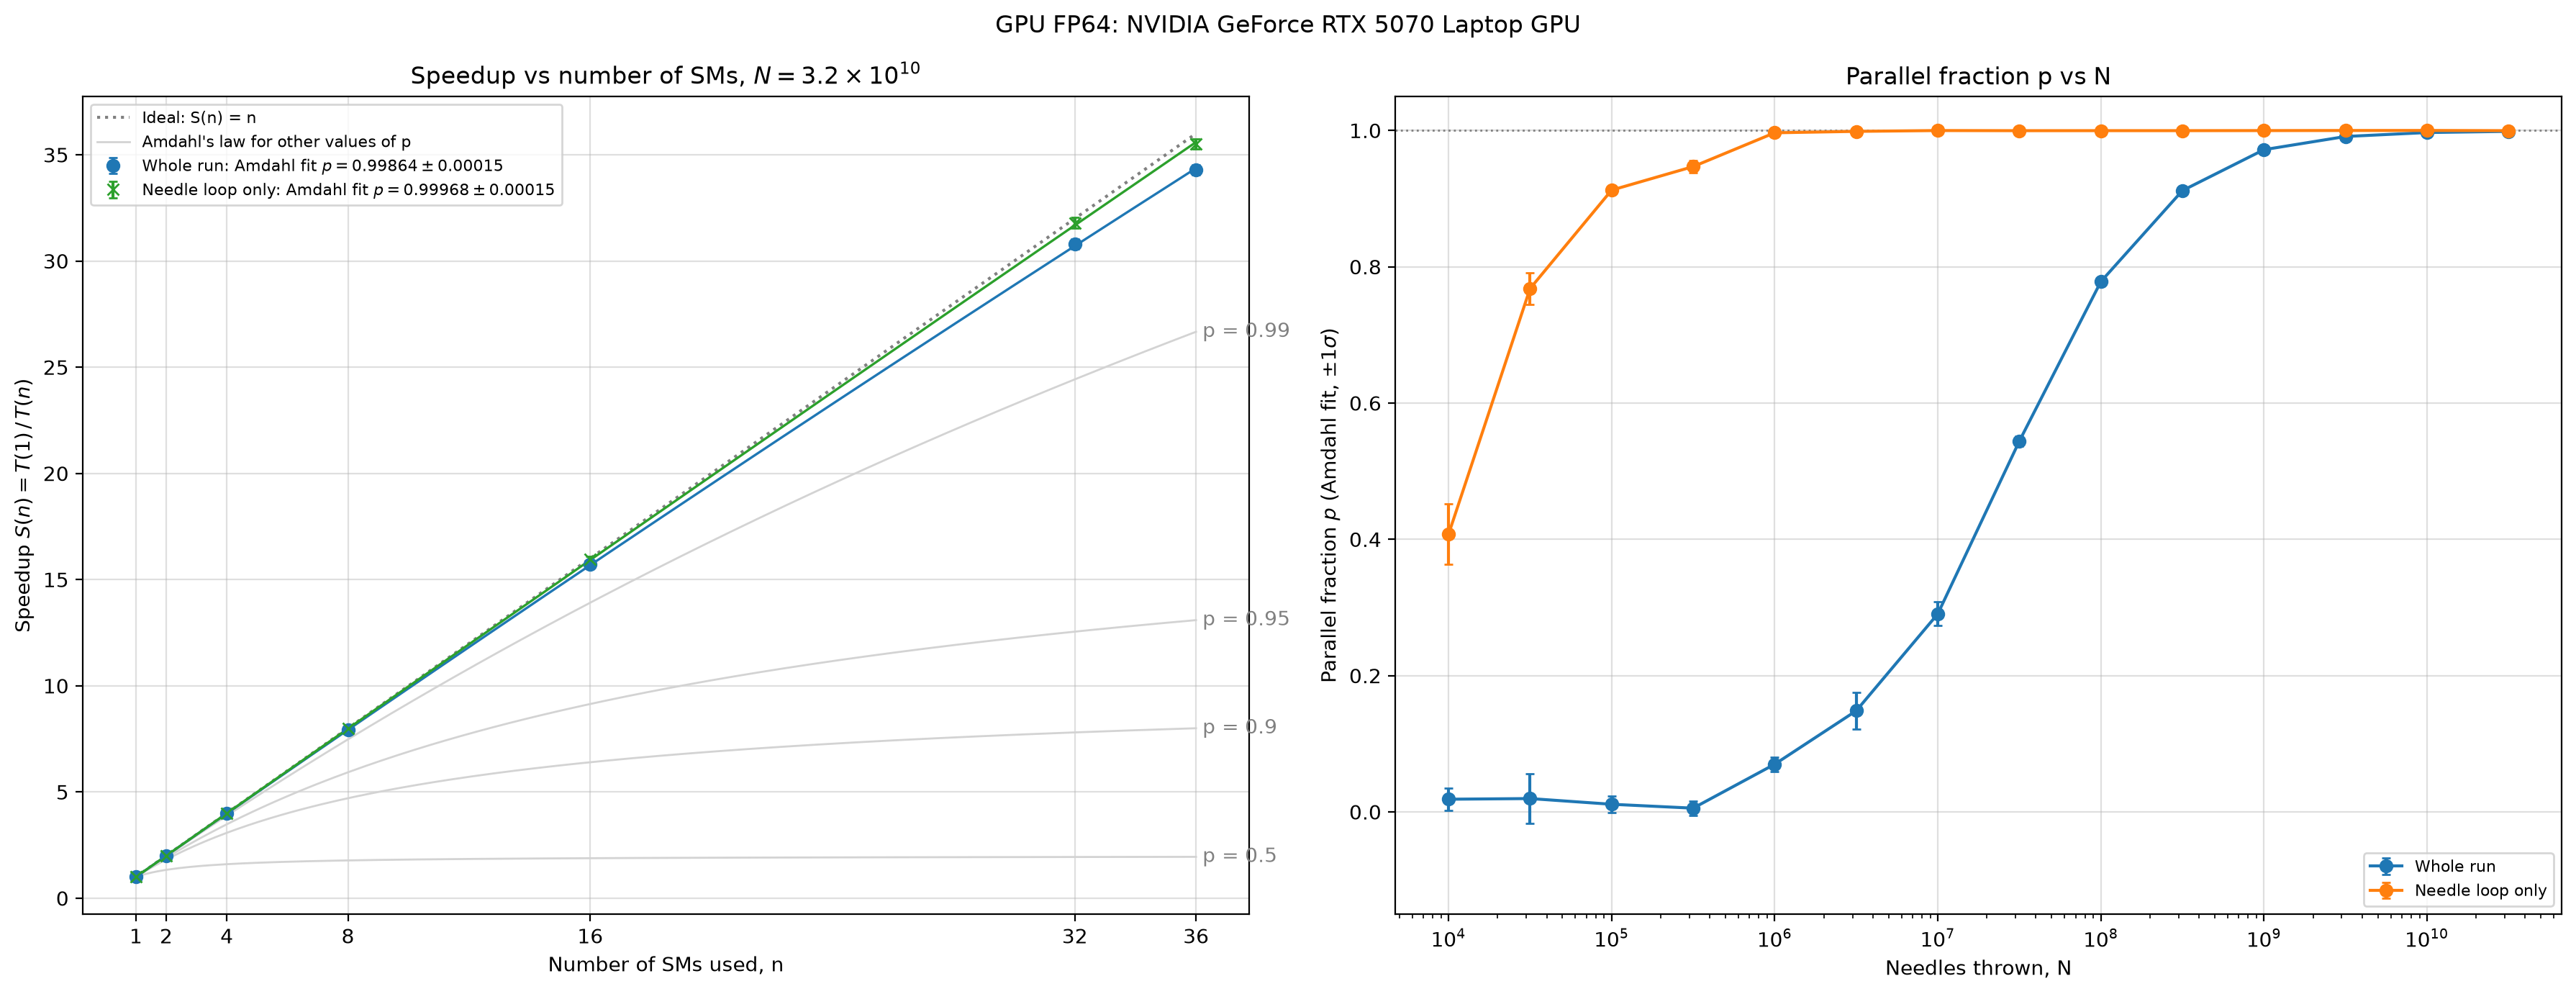
\includegraphics[width=\textwidth]{ep3_amdahl.png}
  \small $N = 3{,}2\times10^{10}$ (FP64): \textbf{34,3× em 36 SMs}, $p = 0{,}9986$; a parte serial é 0,15 s (criar o contexto CUDA)
\end{frame}

% ============================================================ 7. mais fundo

\begin{frame}{Registradores decidem quantos warps cabem}
  \centering\large
  warps que cabem $= \dfrac{65\,536 \text{ registradores por SM}}{\text{registradores por thread} \times 32}$
  \vfill
  \normalsize
  \begin{tabular}{llll}
    \toprule
    & registradores & warps & ocupação \\
    \midrule
    estrela FP64 (laptop) & 80 & 24 de 48 & 0,50 \\
    estrela FP32 (laptop) & 67 & 28 de 48 & 0,58 \\
    estrela FP64 (A30) & 96 & 21 de 64 & \aaa{medida} \\
    \bottomrule
  \end{tabular}
\end{frame}

\begin{frame}{Mais ocupação não é mais rápido (aqui)}
  \centering
  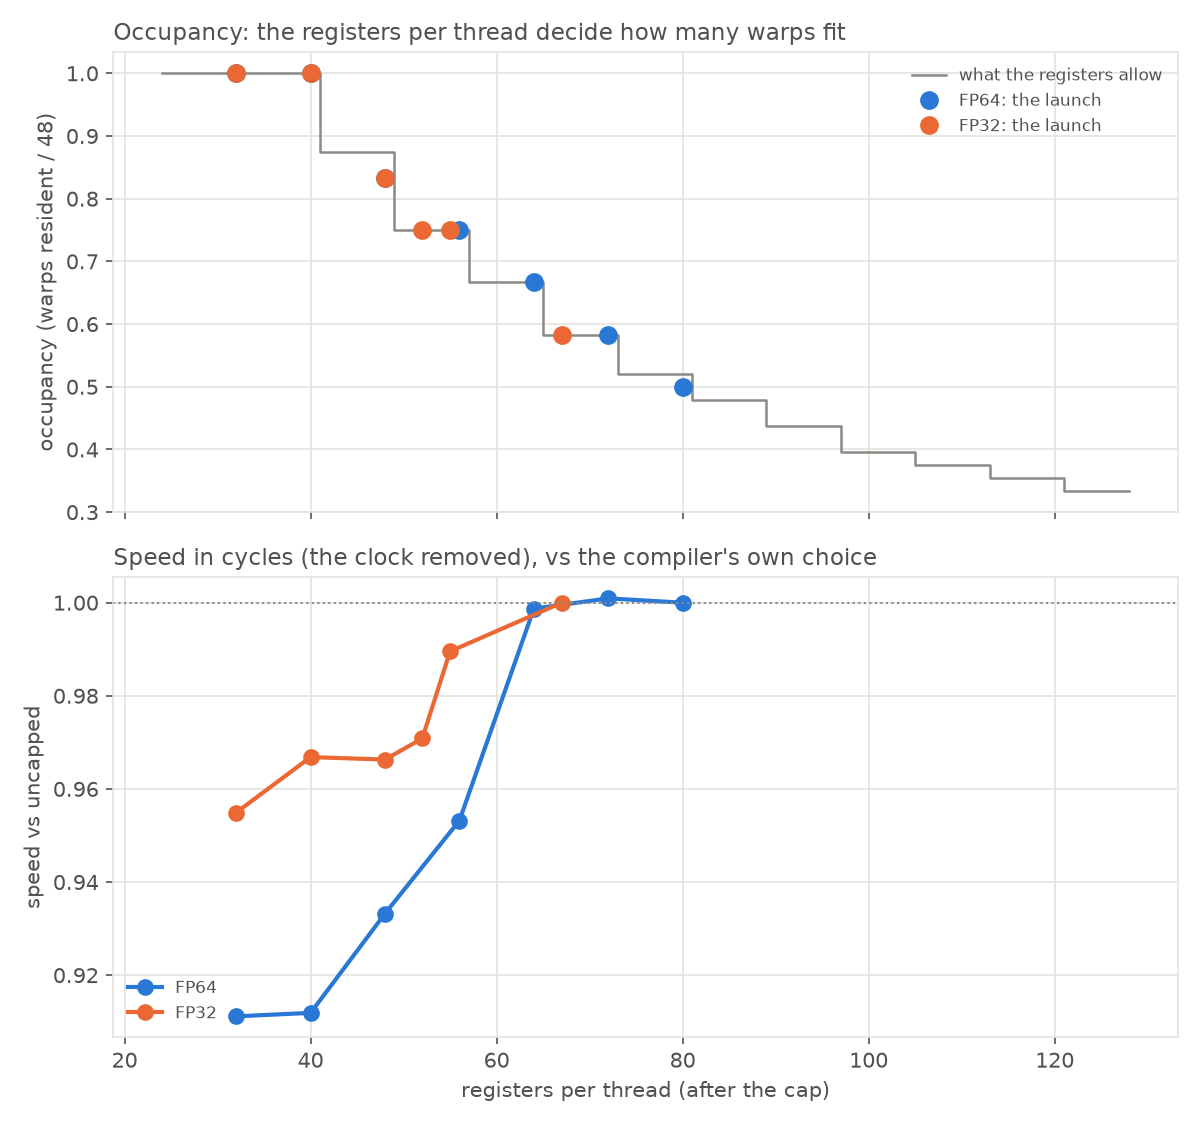
\includegraphics[height=0.75\textheight]{registers_and_occupancy.png}
  \small Limitar os registradores enche o SM, mas o compilador acrescenta instruções e depois derrama valores na memória.
  \aaa{e na A30?}
\end{frame}

% ============================================================ 8. EP4: o código

\begin{frame}{EP4: a estrela manchada}
  \begin{columns}[c]
    \begin{column}{0.4\textwidth}
      \centering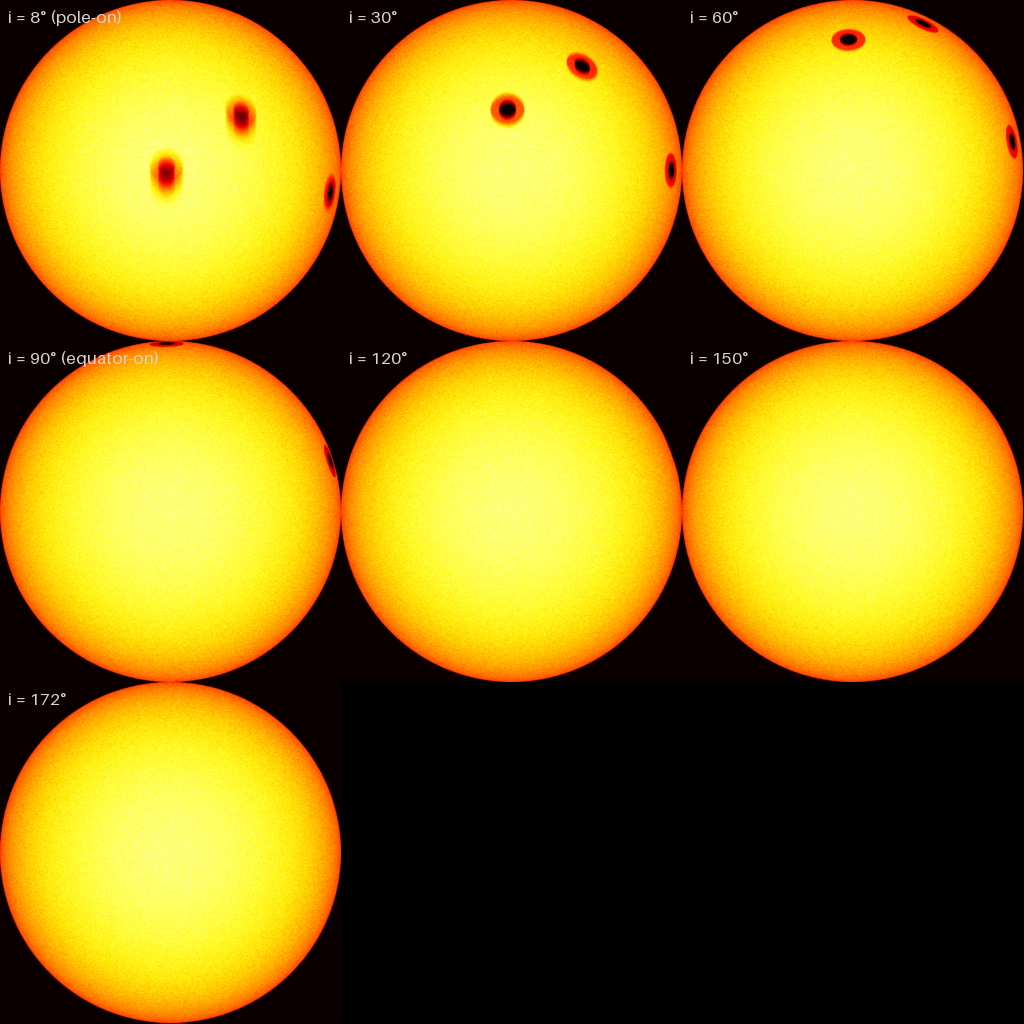
\includegraphics[width=\linewidth]{grid_still.png}
    \end{column}
    \begin{column}{0.57\textwidth}
      \begin{itemize}
        \item um fóton sai da superfície (escurecimento de limbo)
        \item pode cair numa mancha
        \item escapa numa direção: ela escolhe o observador e o quadro
        \item cai num pixel
      \end{itemize}
      \vfill
      O algoritmo é o do EP2; o EP4 o leva para a GPU.
    \end{column}
  \end{columns}
\end{frame}

\begin{frame}[fragile]{EP4: o esqueleto do Buffon, com outro corpo}
  \begin{lstlisting}
__device__ void trace_chunk(long long chunk, ...) {
    curand_init(work.seed, chunk, 0, &rng);           // o mesmo fluxo por pedaço
    for (long long photon = first; photon < end; photon++) {
        long long pixel = trace_photon(&gpu_scene, &rng);  // a física: a mesma função na CPU
        tally_photon(pixel, image, &tallies);         // atomicAdd na imagem (memória global)
    }
}
  \end{lstlisting}
  \vfill
  \begin{itemize}
    \item a descrição da estrela em memória \textbf{constante}
    \item a física compilada para CPU e GPU (\texttt{\_\_host\_\_ \_\_device\_\_})
  \end{itemize}
\end{frame}

\begin{frame}{EP4: a GPU dá os mesmos bits que a CPU}
  \centering
  \begin{tabular}{ll}
    \toprule
    teste & resultado \\
    \midrule
    GPU vs CPU, mesmos fótons, FP64 & \textbf{idênticas, bit a bit} \\
    GPU vs CPU, fótons independentes & $\chi^2/\text{gl} = 0{,}99$ \\
    FP32 vs FP64 & $7\times10^{-4}$ dos fótons mudam de pixel \\
    & (menos que o ruído) \\
    \bottomrule
  \end{tabular}
  \vfill
  Mesmos números aleatórios (Philox, um fluxo por pedaço) e a mesma física: o mesmo resultado.
\end{frame}

% ============================================================ 9. EP4: Amdahl

\begin{frame}{EP4: para onde vai o tempo}
  \centering
  \begin{tabular}{lrrl}
    \toprule
    FP64, $N = 4\times10^{9}$, imagem 1024² (5 GB) & 1 SM & 36 SMs & \\
    \midrule
    fótons & 216,9 s & 6,0 s & 36× \\
    preparar + copiar + \textbf{salvar 5 GB} & 5,6 s & 5,6 s & 1× \\
    \midrule
    execução inteira & 223,5 s & 11,6 s & \textbf{19×} \\
    \bottomrule
  \end{tabular}
  \vfill
  \textbf{A parte serial de uma imagem de alta resolução é a própria imagem.}
\end{frame}

\begin{frame}{O teto de Amdahl}
  \centering
  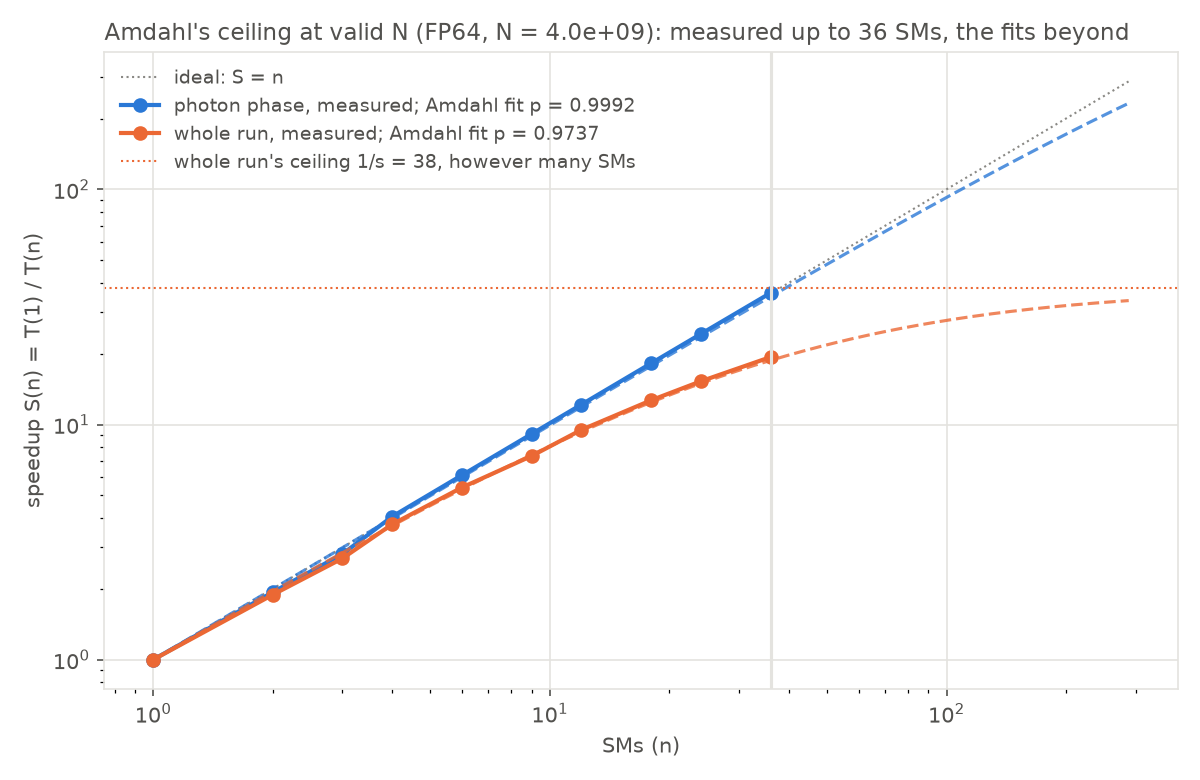
\includegraphics[height=0.8\textheight]{amdahl_ceiling_fp64.png}
\end{frame}

\begin{frame}{Quanto maior $N$, mais perto do ideal}
  \centering
  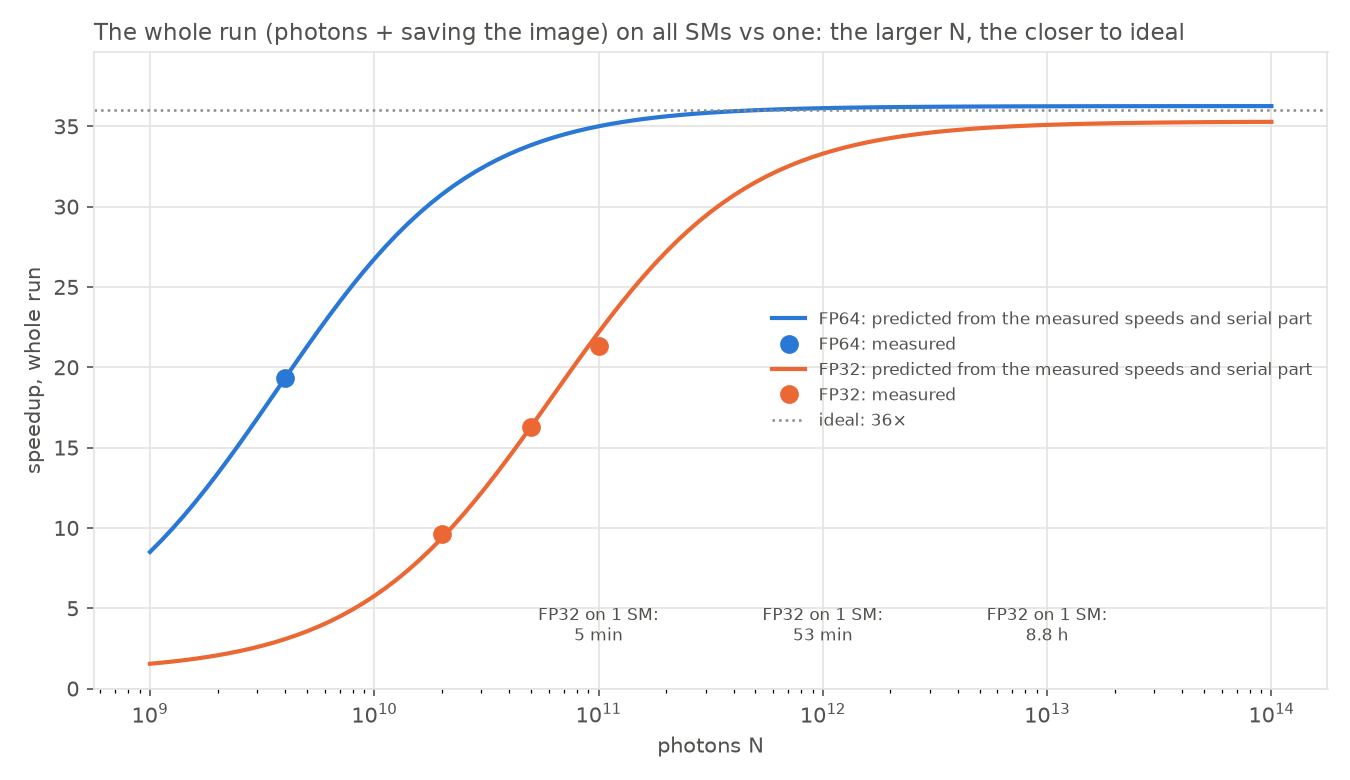
\includegraphics[height=0.8\textheight]{costs_large_n.png}
\end{frame}

\begin{frame}{A mesma lei, outra parte serial}
  \centering
  \begin{tabular}{llll}
    \toprule
    & parte serial & $p$ & 36 SMs \\
    \midrule
    EP3, Buffon & 0,15 s (contexto CUDA) & 0,9986 & 34× \\
    EP4, estrela 1024² & 5,6 s (salvar 5 GB) & 0,974 & 19× \\
    \bottomrule
  \end{tabular}
\end{frame}

\begin{frame}{O laptop e a A30}
  \centering
  \begin{tabular}{lll}
    \toprule
    & laptop (36 SMs) & A30 (56 SMs) \\
    \midrule
    fótons/s, FP32 & $1{,}1\times10^{10}$ & \aaa{} \\
    fótons/s, FP64 & $6{,}7\times10^{8}$ & \aaa{} \\
    FP32 / FP64 & 16,6× & \aaa{} \\
    todos os SMs vs um SM (FP64) & 36,3× & \aaa{} \\
    execução inteira, 1024² & 19× & \aaa{} \\
    \bottomrule
  \end{tabular}
\end{frame}

\begin{frame}{Uma comparação justa: a unidade é o SM}
  \begin{itemize}
    \item ``a GPU é 100× mais rápida que a CPU'': uma GPU inteira contra \textbf{um} núcleo de um código sequencial
    \item é o erro clássico (Lee et al., ISCA 2010)
    \item aqui: a GPU contra ela mesma, um SM e depois todos
    \item a CPU serve para outra coisa: conferir que a GPU dá a resposta certa
  \end{itemize}
\end{frame}

% ============================================================ 10. resultado e fechamento

\begin{frame}{Mais fótons, imagem mais limpa: SNR $\propto \sqrt{N}$}
  \centering
  \animategraphics[controls,loop,width=0.95\textwidth]{15}{frames/ladder-}{001}{150}
  \small as manchas aparecem entre $10^9$ e $10^{10}$ fótons
\end{frame}

\begin{frame}{Três lições}
  \begin{enumerate}
    \item A GPU vence quando o trabalho são muitos pedaços independentes.
    \item Primeiro a correção: os mesmos bits na CPU e na GPU.
    \item Amdahl decide: ache a parte serial (o contexto, a imagem), meça a execução inteira e diga contra o quê cada aceleração foi medida.
  \end{enumerate}
\end{frame}

\begin{frame}
  \centering\Large Obrigado!\\[1em]
  \normalsize Perguntas?
\end{frame}

\end{document}
